%!TeX root=../houndtop.tex
\chapter{The Hound of the Baskervilles}
\lettrine[lines=4]{O}{ne} of Sherlock Holmes's defects—if, indeed, one may call it a defect—was that he was exceedingly loath to communicate his full plans to any other person until the instant of their fulfilment. Partly it came no doubt from his own masterful nature, which loved to dominate and surprise those who were around him. Partly also from his professional caution, which urged him never to take any chances. The result, however, was very trying for those who were acting as his agents and assistants. I had often suffered under it, but never more so than during that long drive in the darkness. The great ordeal was in front of us; at last we were about to make our final effort, and yet Holmes had said nothing, and I could only surmise what his course of action would be. My nerves thrilled with anticipation when at last the cold wind upon our faces and the dark, void spaces on either side of the narrow road told me that we were back upon the moor once again. Every stride of the horses and every turn of the wheels was taking us nearer to our supreme adventure.

Our conversation was hampered by the presence of the driver of the hired wagonette, so that we were forced to talk of trivial matters when our nerves were tense with emotion and anticipation. It was a relief to me, after that unnatural restraint, when we at last passed Frankland's house and knew that we were drawing near to the Hall and to the scene of action. We did not drive up to the door but got down near the gate of the avenue. The wagonette was paid off and ordered to return to Coombe Tracey forthwith, while we started to walk to Merripit House.

»Are you armed, Lestrade?«

The little detective smiled.

»As long as I have my trousers I have a hip-pocket, and as long as I have my hip-pocket I have something in it.«

»Good! My friend and I are also ready for emergencies.«

»You're mighty close about this affair, Mr Holmes. What's the game now?«

»A waiting game.«

»My word, it does not seem a very cheerful place,« said the detective with a shiver, glancing round him at the gloomy slopes of the hill and at the huge lake of fog which lay over the Grimpen Mire. »I see the lights of a house ahead of us.«

»That is Merripit House and the end of our journey. I must request you to walk on tiptoe and not to talk above a whisper.«

We moved cautiously along the track as if we were bound for the house, but Holmes halted us when we were about two hundred yards from it.

»This will do,« said he. »These rocks upon the right make an admirable screen.«

»We are to wait here?«

»Yes, we shall make our little ambush here. Get into this hollow, Lestrade. You have been inside the house, have you not, Watson? Can you tell the position of the rooms? What are those latticed windows at this end?«

»I think they are the kitchen windows.«

»And the one beyond, which shines so brightly?«

»That is certainly the dining-room.«

»The blinds are up. You know the lie of the land best. Creep forward quietly and see what they are doing—but for heaven's sake don't let them know that they are watched!«

I tiptoed down the path and stooped behind the low wall which surrounded the stunted orchard. Creeping in its shadow I reached a point whence I could look straight through the uncurtained window.

There were only two men in the room, Sir Henry and Stapleton. They sat with their profiles towards me on either side of the round table. Both of them were smoking cigars, and coffee and wine were in front of them. Stapleton was talking with animation, but the baronet looked pale and distrait. Perhaps the thought of that lonely walk across the ill-omened moor was weighing heavily upon his mind.

As I watched them Stapleton rose and left the room, while Sir Henry filled his glass again and leaned back in his chair, puffing at his cigar. I heard the creak of a door and the crisp sound of boots upon gravel. The steps passed along the path on the other side of the wall under which I crouched. Looking over, I saw the naturalist pause at the door of an out-house in the corner of the orchard. A key turned in a lock, and as he passed in there was a curious scuffling noise from within. He was only a minute or so inside, and then I heard the key turn once more and he passed me and re-entered the house. I saw him rejoin his guest, and I crept quietly back to where my companions were waiting to tell them what I had seen.

»You say, Watson, that the lady is not there?« Holmes asked, when I had finished my report.

»No.«

»Where can she be, then, since there is no light in any other room except the kitchen?«

»I cannot think where she is.«

I have said that over the great Grimpen Mire there hung a dense, white fog. It was drifting slowly in our direction, and banked itself up like a wall on that side of us, low, but thick and well defined. The moon shone on it, and it looked like a great shimmering ice-field, with the heads of the distant tors as rocks borne upon its surface. Holmes's face was turned towards it, and he muttered impatiently as he watched its sluggish drift.

»It's moving towards us, Watson.«

»Is that serious?«

»Very serious, indeed—the one thing upon earth which could have disarranged my plans. He can't be very long, now. It is already ten o'clock. Our success and even his life may depend upon his coming out before the fog is over the path.«

The night was clear and fine above us. The stars shone cold and bright, while a half-moon bathed the whole scene in a soft, uncertain light. Before us lay the dark bulk of the house, its serrated roof and bristling chimneys hard outlined against the silver-spangled sky. Broad bars of golden light from the lower windows stretched across the orchard and the moor. One of them was suddenly shut off. The servants had left the kitchen. There only remained the lamp in the dining-room where the two men, the murderous host and the unconscious guest, still chatted over their cigars.

Every minute that white woolly plain which covered one half of the moor was drifting closer and closer to the house. Already the first thin wisps of it were curling across the golden square of the lighted window. The farther wall of the orchard was already invisible, and the trees were standing out of a swirl of white vapour. As we watched it the fog-wreaths came crawling round both corners of the house and rolled slowly into one dense bank, on which the upper floor and the roof floated like a strange ship upon a shadowy sea. Holmes struck his hand passionately upon the rock in front of us and stamped his feet in his impatience.

»If he isn't out in a quarter of an hour the path will be covered. In half an hour we won't be able to see our hands in front of us.«

»Shall we move farther back upon higher ground?«

»Yes, I think it would be as well.«

So as the fog-bank flowed onward we fell back before it until we were half a mile from the house, and still that dense white sea, with the moon silvering its upper edge, swept slowly and inexorably on.

»We are going too far,« said Holmes. »We dare not take the chance of his being overtaken before he can reach us. At all costs we must hold our ground where we are.« He dropped on his knees and clapped his ear to the ground. »Thank God, I think that I hear him coming.«

A sound of quick steps broke the silence of the moor. Crouching among the stones we stared intently at the silver-tipped bank in front of us. The steps grew louder, and through the fog, as through a curtain, there stepped the man whom we were awaiting. He looked round him in surprise as he emerged into the clear, starlit night. Then he came swiftly along the path, passed close to where we lay, and went on up the long slope behind us. As he walked he glanced continually over either shoulder, like a man who is ill at ease.

\begin{figure}[tbph]
\centering

\includegraphics[width=\linewidth]{14_lookedround}
\caption{He looked round him in surprise.}
\end{figure}

»Hist!« cried Holmes, and I heard the sharp click of a cocking pistol. »Look out! It's coming!«

There was a thin, crisp, continuous patter from somewhere in the heart of that crawling bank. The cloud was within fifty yards of where we lay, and we glared at it, all three, uncertain what horror was about to break from the heart of it. I was at Holmes's elbow, and I glanced for an instant at his face. It was pale and exultant, his eyes shining brightly in the moonlight. But suddenly they started forward in a rigid, fixed stare, and his lips parted in amazement. At the same instant Lestrade gave a yell of terror and threw himself face downward upon the ground. I sprang to my feet, my inert hand grasping my pistol, my mind paralysed by the dreadful shape which had sprung out upon us from the shadows of the fog. A hound it was, an enormous coal-black hound, but not such a hound as mortal eyes have ever seen. Fire burst from its open mouth, its eyes glowed with a smouldering glare, its muzzle and hackles and dewlap were outlined in flickering flame. Never in the delirious dream of a disordered brain could anything more savage, more appalling, more hellish be conceived than that dark form and savage face which broke upon us out of the wall of fog.

\begin{figure}[tbph]
\centering
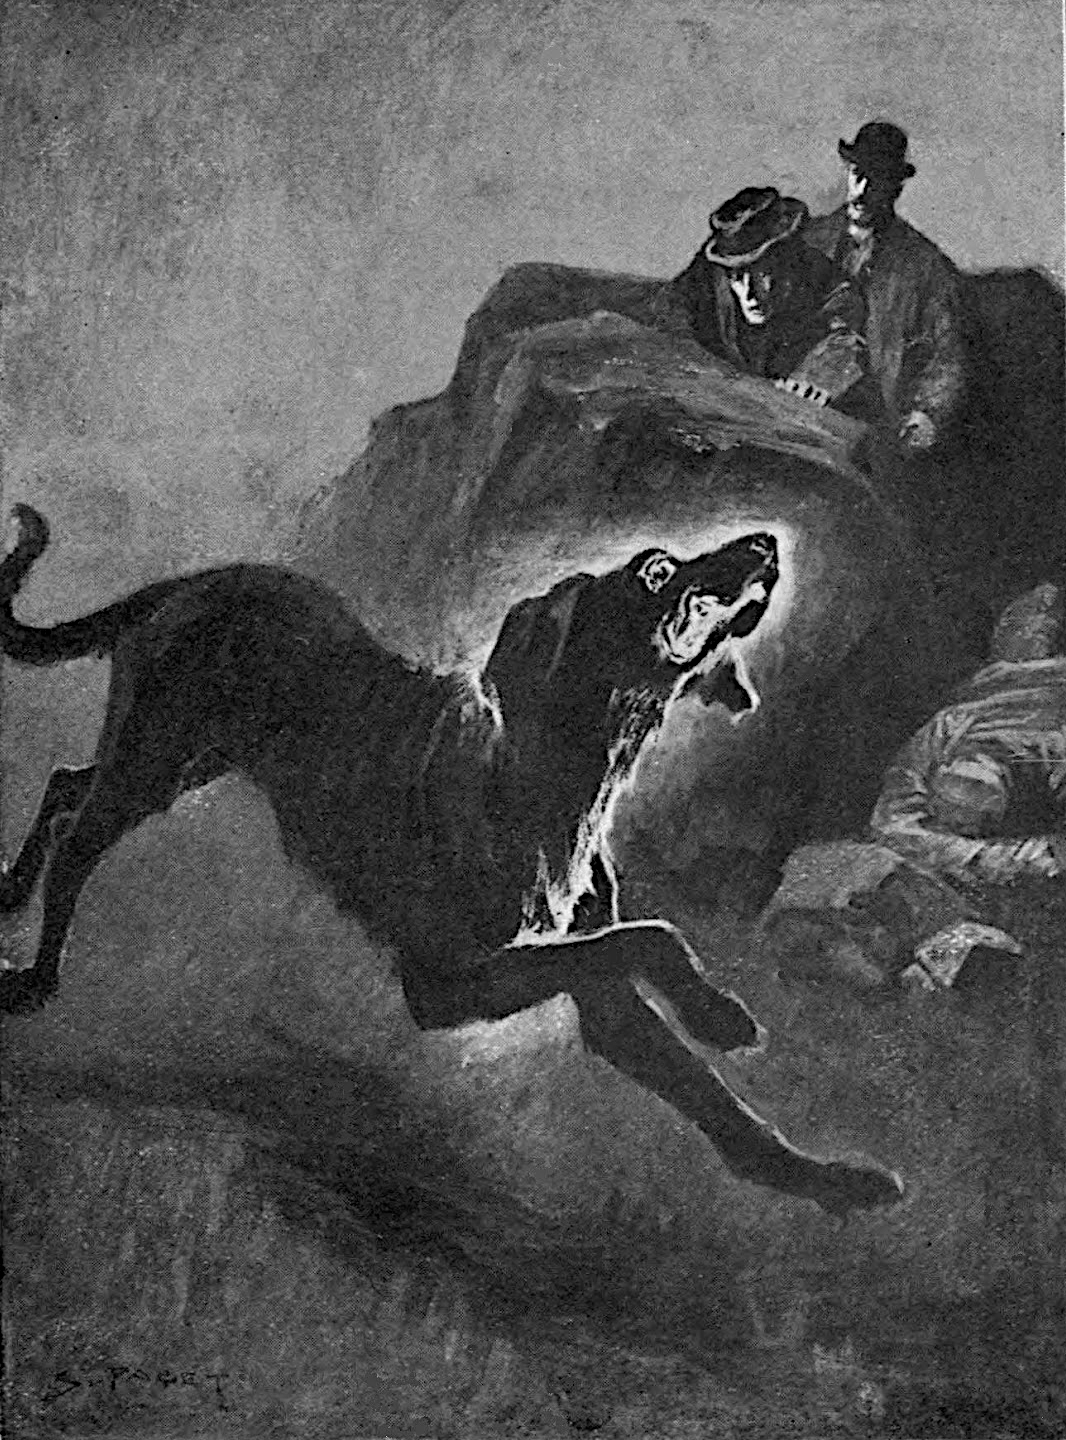
\includegraphics[width=\linewidth]{14_thehound}
\caption{The Hound of the Baskervilles}
\end{figure}

With long bounds the huge black creature was leaping down the track, following hard upon the footsteps of our friend. So paralysed were we by the apparition that we allowed him to pass before we had recovered our nerve. Then Holmes and I both fired together, and the creature gave a hideous howl, which showed that one at least had hit him. He did not pause, however, but bounded onward. Far away on the path we saw Sir Henry looking back, his face white in the moonlight, his hands raised in horror, glaring helplessly at the frightful thing which was hunting him down.

But that cry of pain from the hound had blown all our fears to the winds. If he was vulnerable he was mortal, and if we could wound him we could kill him. Never have I seen a man run as Holmes ran that night. I am reckoned fleet of foot, but he outpaced me as much as I outpaced the little professional. In front of us as we flew up the track we heard scream after scream from Sir Henry and the deep roar of the hound. I was in time to see the beast spring upon its victim, hurl him to the ground, and worry at his throat. But the next instant Holmes had emptied five barrels of his revolver into the creature's flank. With a last howl of agony and a vicious snap in the air, it rolled upon its back, four feet pawing furiously, and then fell limp upon its side. I stooped, panting, and pressed my pistol to the dreadful, shimmering head, but it was useless to press the trigger. The giant hound was dead.



Sir Henry lay insensible where he had fallen. We tore away his collar, and Holmes breathed a prayer of gratitude when we saw that there was no sign of a wound and that the rescue had been in time. Already our friend's eyelids shivered and he made a feeble effort to move. Lestrade thrust his brandy-flask between the baronet's teeth, and two frightened eyes were looking up at us.

»My God!« he whispered. »What was it? What, in heaven's name, was it?«

»It's dead, whatever it is,« said Holmes. »We've laid the family ghost once and forever.«

In mere size and strength it was a terrible creature which was lying stretched before us. It was not a pure bloodhound and it was not a pure mastiff; but it appeared to be a combination of the two—gaunt, savage, and as large as a small lioness. Even now, in the stillness of death, the huge jaws seemed to be dripping with a bluish flame and the small, deep-set, cruel eyes were ringed with fire. I placed my hand upon the glowing muzzle, and as I held them up my own fingers smouldered and gleamed in the darkness.

\begin{figure}[tbph]
\centering
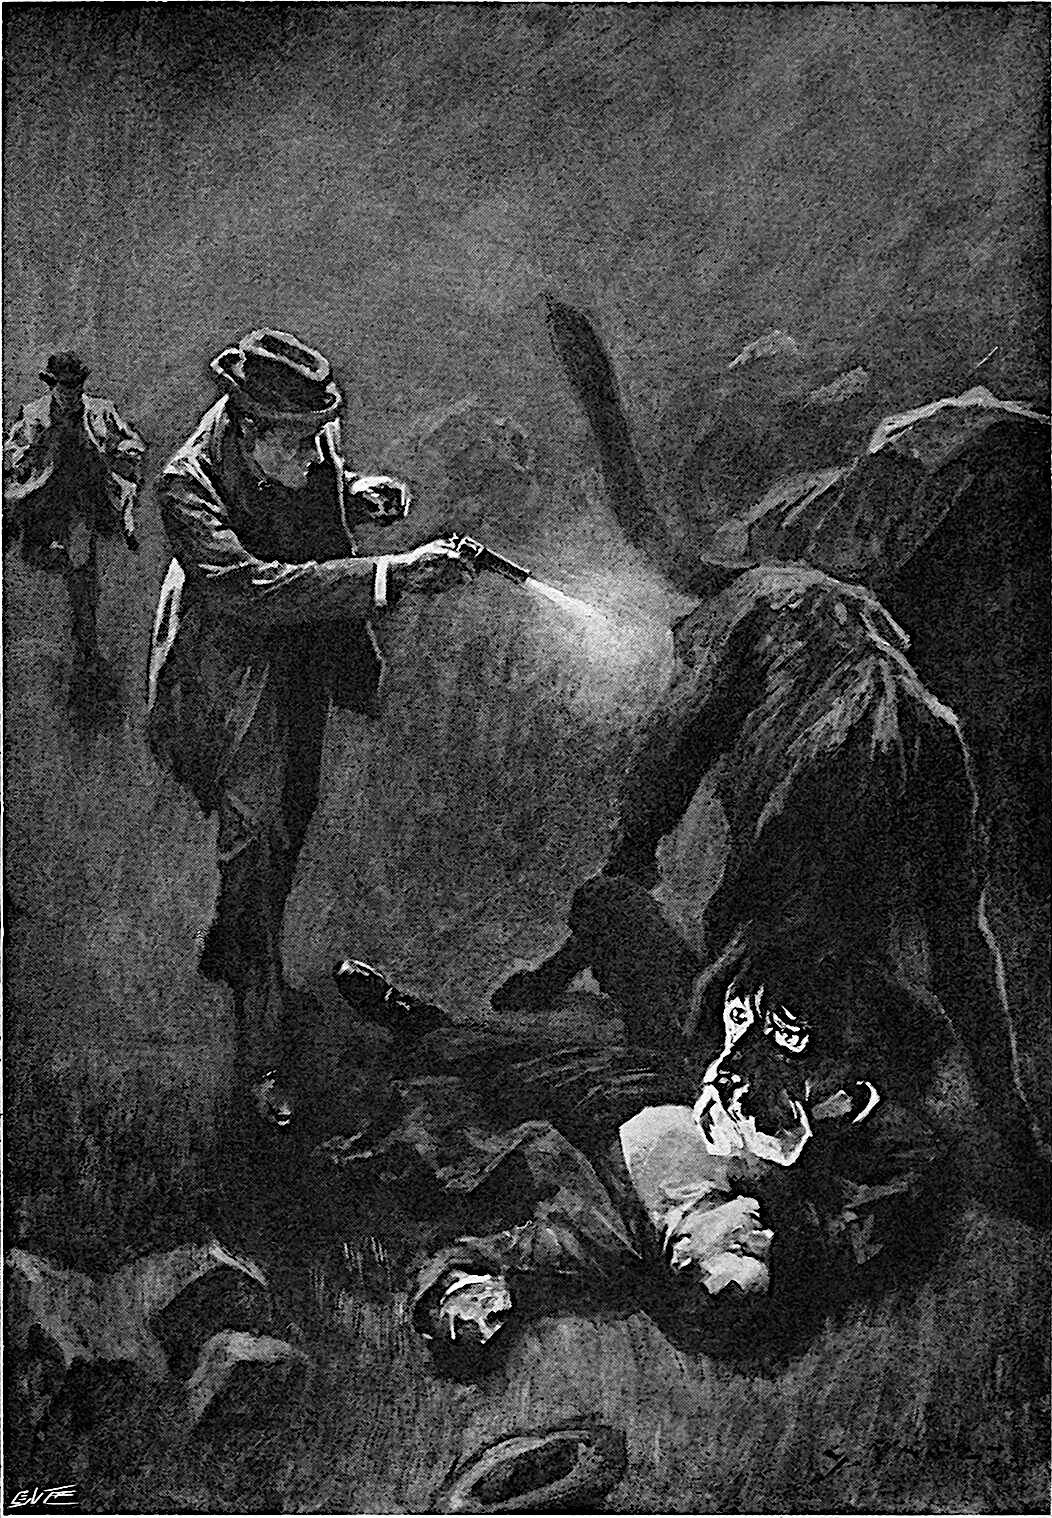
\includegraphics[width=\linewidth]{14_hounddead}
\caption{Holmes emptied five barrels of his revolver into the creature's flank}
\end{figure}

»Phosphorus,« I said.

»A cunning preparation of it,« said Holmes, sniffing at the dead animal. »There is no smell which might have interfered with his power of scent. We owe you a deep apology, Sir Henry, for having exposed you to this fright. I was prepared for a hound, but not for such a creature as this. And the fog gave us little time to receive him.«

»You have saved my life.«

»Having first endangered it. Are you strong enough to stand?«

»Give me another mouthful of that brandy and I shall be ready for anything. So! Now, if you will help me up. What do you propose to do?«

»To leave you here. You are not fit for further adventures to-night. If you will wait, one or other of us will go back with you to the Hall.«

He tried to stagger to his feet; but he was still ghastly pale and trembling in every limb. We helped him to a rock, where he sat shivering with his face buried in his hands.

»We must leave you now,« said Holmes. »The rest of our work must be done, and every moment is of importance. We have our case, and now we only want our man.«

»It's a thousand to one against our finding him at the house,« he continued as we retraced our steps swiftly down the path. »Those shots must have told him that the game was up.«

»We were some distance off, and this fog may have deadened them.«

»He followed the hound to call him off—of that you may be certain. No, no, he's gone by this time! But we'll search the house and make sure.«

The front door was open, so we rushed in and hurried from room to room to the amazement of a doddering old manservant, who met us in the passage. There was no light save in the dining-room, but Holmes caught up the lamp and left no corner of the house unexplored. No sign could we see of the man whom we were chasing. On the upper floor, however, one of the bedroom doors was locked.

»There's someone in here,« cried Lestrade. »I can hear a movement. Open this door!«

A faint moaning and rustling came from within. Holmes struck the door just over the lock with the flat of his foot and it flew open. Pistol in hand, we all three rushed into the room.

But there was no sign within it of that desperate and defiant villain whom we expected to see. Instead we were faced by an object so strange and so unexpected that we stood for a moment staring at it in amazement.

The room had been fashioned into a small museum, and the walls were lined by a number of glass-topped cases full of that collection of butterflies and moths the formation of which had been the relaxation of this complex and dangerous man. In the centre of this room there was an upright beam, which had been placed at some period as a support for the old worm-eaten baulk of timber which spanned the roof. To this post a figure was tied, so swathed and muffled in the sheets which had been used to secure it that one could not for the moment tell whether it was that of a man or a woman. One towel passed round the throat and was secured at the back of the pillar. Another covered the lower part of the face, and over it two dark eyes—eyes full of grief and shame and a dreadful questioning—stared back at us. In a minute we had torn off the gag, unswathed the bonds, and Mrs Stapleton sank upon the floor in front of us. As her beautiful head fell upon her chest I saw the clear red weal of a whiplash across her neck.

»The brute!« cried Holmes. »Here, Lestrade, your brandy-bottle! Put her in the chair! She has fainted from ill-usage and exhaustion.«

She opened her eyes again.

\begin{figure}[tbph]
\centering
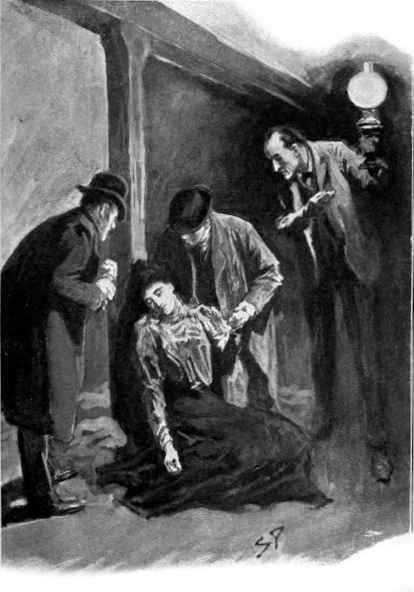
\includegraphics[width=\linewidth]{14_swoon}
\caption{Mrs Stapleton sank upon the floor}
\end{figure}

»Is he safe?« she asked. »Has he escaped?«

»He cannot escape us, madam.«

»No, no, I did not mean my husband. Sir Henry? Is he safe?«

»Yes.«

»And the hound?«

»It is dead.«

She gave a long sigh of satisfaction.

»Thank God! Thank God! Oh, this villain! See how he has treated me!« She shot her arms out from her sleeves, and we saw with horror that they were all mottled with bruises. »But this is nothing—nothing! It is my mind and soul that he has tortured and defiled. I could endure it all, ill-usage, solitude, a life of deception, everything, as long as I could still cling to the hope that I had his love, but now I know that in this also I have been his dupe and his tool.« She broke into passionate sobbing as she spoke.

»You bear him no good will, madam,« said Holmes. »Tell us then where we shall find him. If you have ever aided him in evil, help us now and so atone.«

»There is but one place where he can have fled,« she answered. »There is an old tin mine on an island in the heart of the mire. It was there that he kept his hound and there also he had made preparations so that he might have a refuge. That is where he would fly.«

The fog-bank lay like white wool against the window. Holmes held the lamp towards it.

»See,« said he. »No one could find his way into the Grimpen Mire to-night.«

She laughed and clapped her hands. Her eyes and teeth gleamed with fierce merriment.

»He may find his way in, but never out,« she cried. »How can he see the guiding wands to-night? We planted them together, he and I, to mark the pathway through the mire. Oh, if I could only have plucked them out to-day. Then indeed you would have had him at your mercy!«

It was evident to us that all pursuit was in vain until the fog had lifted. Meanwhile we left Lestrade in possession of the house while Holmes and I went back with the baronet to Baskerville Hall. The story of the Stapletons could no longer be withheld from him, but he took the blow bravely when he learned the truth about the woman whom he had loved. But the shock of the night's adventures had shattered his nerves, and before morning he lay delirious in a high fever, under the care of Dr Mortimer. The two of them were destined to travel together round the world before Sir Henry had become once more the hale, hearty man that he had been before he became master of that ill-omened estate.

And now I come rapidly to the conclusion of this singular narrative, in which I have tried to make the reader share those dark fears and vague surmises which clouded our lives so long and ended in so tragic a manner. On the morning after the death of the hound the fog had lifted and we were guided by Mrs Stapleton to the point where they had found a pathway through the bog. It helped us to realize the horror of this woman's life when we saw the eagerness and joy with which she laid us on her husband's track. We left her standing upon the thin peninsula of firm, peaty soil which tapered out into the widespread bog. From the end of it a small wand planted here and there showed where the path zigzagged from tuft to tuft of rushes among those green-scummed pits and foul quagmires which barred the way to the stranger. Rank reeds and lush, slimy water-plants sent an odour of decay and a heavy miasmatic vapour onto our faces, while a false step plunged us more than once thigh-deep into the dark, quivering mire, which shook for yards in soft undulations around our feet. Its tenacious grip plucked at our heels as we walked, and when we sank into it it was as if some malignant hand was tugging us down into those obscene depths, so grim and purposeful was the clutch in which it held us. Once only we saw a trace that someone had passed that perilous way before us. From amid a tuft of cotton grass which bore it up out of the slime some dark thing was projecting. Holmes sank to his waist as he stepped from the path to seize it, and had we not been there to drag him out he could never have set his foot upon firm land again. He held an old black boot in the air. »Meyers, Toronto,« was printed on the leather inside.

»It is worth a mud bath,« said he. »It is our friend Sir Henry's missing boot.«

»Thrown there by Stapleton in his flight.«

»Exactly. He retained it in his hand after using it to set the hound upon the track. He fled when he knew the game was up, still clutching it. And he hurled it away at this point of his flight. We know at least that he came so far in safety.«

But more than that we were never destined to know, though there was much which we might surmise. There was no chance of finding footsteps in the mire, for the rising mud oozed swiftly in upon them, but as we at last reached firmer ground beyond the morass we all looked eagerly for them. But no slightest sign of them ever met our eyes. If the earth told a true story, then Stapleton never reached that island of refuge towards which he struggled through the fog upon that last night. Somewhere in the heart of the great Grimpen Mire, down in the foul slime of the huge morass which had sucked him in, this cold and cruel-hearted man is forever buried.

\begin{figure}[h!]
\centering

\includegraphics[width=0.8\linewidth]{14_creatureconfined}
\caption{Where the animal had been confined}
\end{figure}

Many traces we found of him in the bog-girt island where he had hid his savage ally. A huge driving-wheel and a shaft half-filled with rubbish showed the position of an abandoned mine. Beside it were the crumbling remains of the cottages of the miners, driven away no doubt by the foul reek of the surrounding swamp. In one of these a staple and chain with a quantity of gnawed bones showed where the animal had been confined. A skeleton with a tangle of brown hair adhering to it lay among the \textit{débris.}

»A dog!« said Holmes. »By Jove, a curly-haired spaniel. Poor Mortimer will never see his pet again. Well, I do not know that this place contains any secret which we have not already fathomed. He could hide his hound, but he could not hush its voice, and hence came those cries which even in daylight were not pleasant to hear. On an emergency he could keep the hound in the out-house at Merripit, but it was always a risk, and it was only on the supreme day, which he regarded as the end of all his efforts, that he dared do it. This paste in the tin is no doubt the luminous mixture with which the creature was daubed. It was suggested, of course, by the story of the family hell-hound, and by the desire to frighten old Sir Charles to death. No wonder the poor devil of a convict ran and screamed, even as our friend did, and as we ourselves might have done, when he saw such a creature bounding through the darkness of the moor upon his track. It was a cunning device, for, apart from the chance of driving your victim to his death, what peasant would venture to inquire too closely into such a creature should he get sight of it, as many have done, upon the moor? I said it in London, Watson, and I say it again now, that never yet have we helped to hunt down a more dangerous man than he who is lying yonder«—he swept his long arm towards the huge mottled expanse of green-splotched bog which stretched away until it merged into the russet slopes of the moor.